\section{Introduction}\label{sec:intro}
\subsection{GIMLi -- concept and overview}\label{sec:gimli}
In geophysics, various physical processes and fields are used to gain information about the subsurface parameters.
The fields and processes can be very well studied and understood by simulation assuming a parameter distribution.
This so-called forward task can be done by using analytical formulae and numerical integration, or numerical schemes deploying finite difference or finite element techniques.
In the recent years, very different studies have been presented that open up new methods to be used.

However, in almost all approaches the task is finally to derive subsurface parameters, i.e. the inverse problem has to be solved.
Very often this is ill-posed, i.e. a variety of solutions is fitting the data within error bounds.
Hence regularization methods have to be applied.
There exist numerous inversion and regularization schemes, which do not have to be reinvented.
Furthermore, often a resolution analysis is required in order to appraise the quality of the results.
The idea of GIMLi is to present a very flexible framework for geophysical inversion and modelling such that it can be used from any forward operator.
All problems such as optimization of regularization parameters, line search are solved generally.
The GIMLi library is structured into four layers (Fig.~\ref{fig:gimliblock}) that are based on each other:

\begin{description}
	\item[The basic layer] holds fundamental algebraic methods and mesh containers for model parameterisation 
	\item[The modelling\&region layer] administrates the modelling classes that are based on a basis class and the connection to constraints and transform functions
	\item[The inversion layer] is a template class for minimisation with different methods, inverse solvers, line search, $\lambda$ optimisation and resolution analysis
	\item[In Inversion frameworks] sophisticated techniques are formulated, e.g. time-lapse strategies, roll-along inversion or different kinds of joint inversion
\end{description}

\begin{figure}[htb]
\centering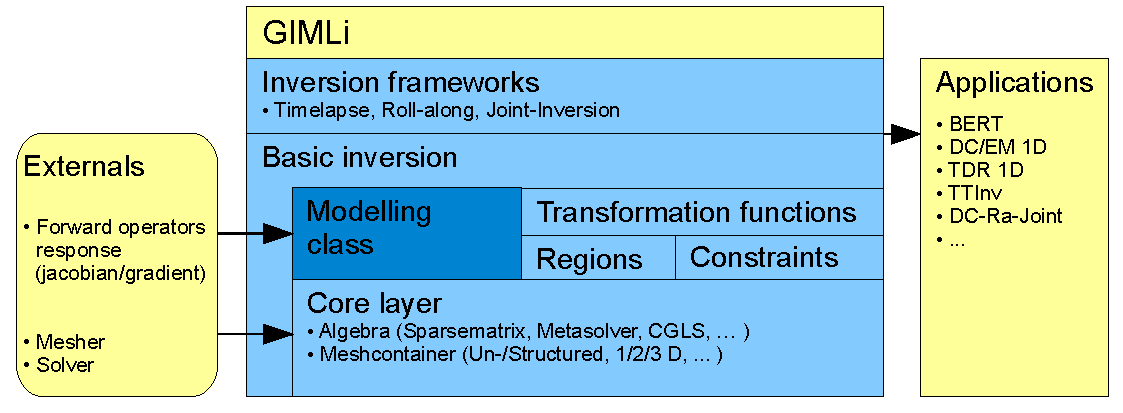
\includegraphics[width=0.85\textwidth]{gimliblock}
\caption{Scheme of the GIMLi library, applications and externals}\label{fig:gimliblock}
\end{figure} 

External programs are, e.g., mesh generators and solvers for linear systems.
For generating quality constrained irregular 2d and 3d meshes, we usually use \cw{Triangle}~\citep{triangle} and \cw{TetGen}~\citep{tetgen}.
For solving linear systems we recommend the open-source collection \cw{SuiteSparse} \citep{davis}, which contains multi-frontal direct\&iterative solvers as well as reordering algorithms.

External forward operators can be easily linked against GIMLi.
As soon they meet the requirements, the inversion can be setup and run with 2 lines.

%%%%%%%%%%%%%%%%%%%%%%%%%%%%%%%%%%%%%%%%%%%%%%%%%%%%%%%%%%%%%%%%%%%%%%%%%%%
\subsection{Minimisation and regularization methods}\label{sec:mini}
Assume we have a discrete number of data $d_i$ assembled in a data vector $\d=[d_1,\ldots,d_D]^T$.
We want to find a parameter distribution represented by a discrete model vector $\m=[m_1,\ldots,m_M]^T$ such that the forwad response $\f(\m)$ approximates $\d$.
To each datum a variance $\delta d_i$ is associated.
By weighting the individual misfit $f_i-d_i$ with $\delta d_i$ we obtain a unit-less misfit vector, such that different data are combined easily.

We try to minimise the misfit vector in a least squares sense using the objective function
\begin{equation}\label{eq:phid}
\Phi_d=\sum\limits_{i=1}{D} \left| \frac{d_i-f_i(\m)}{\delta d_i} \right|^2
= \big\Vert \D(\d - \f(\m)) \big\Vert^2_2 \rightarrow \min
\quad\mbox{with}\quad \D=\mbox{diag}(\delta d_i^{-1})\quad.
\end{equation}

More generally, the inverse data covariance matrix $\W_d^{-1}$ can be used instead of $\D$ if the variances are correlated.
Since the problem is usually non-unique, regularization has to be applied.
We concentrate on explicit and global regularization (CITE) and use a generalized matrix formulation (CITE) to obtain a model objective function 
\begin{equation}\label{eq:phim}
\Phi_m = \|\W^c \C \W^m (\m-\m^R)\|^2_2\quad.
\end{equation}

$\m^R$ represents a reference model.
The matrix $\C$ is a derivative matrix or an identity matrix or a mixture of it.
In the first neighboring relations are taken into account (smoothness constraints), whereas in the latter (zeroth order smoothness) they are not.
The assumption of a smooth model is often the only choice to cope with ill-posedness and limited resolution.
However the degree of smoothness can be controlled flexibly with the mostly diagonal weighting matrices $\W^b=\diag(w^b_i)$ and $\W^m=\diag(w^m_i)$.
A derivative matrix consists of $C$ rows or constraint equations constraining the $M$ model cells corresponding to the rows.
By choosing the $w^m_i$  each model cell can be weighted individually such that a varying degree of smoothness or vicinity to the reference model can be achieved. 
Doing so, parameter constraints are applied using cell-dependent regularization.
On the contrary, we are able to incorporate structural constraints by setting the the weights $w^c_i$ for the individual model boundaries. 
For example, we can allow for arbitrary contrasts along a known boundary (e.g. from seismics or boreholes) in an otherwise smooth model (CITE).

Finally, a regularization parameter $\lambda$ is used to weight $\Phi_d$ and $\Phi_m$ so that we minimize
\begin{equation}\label{eq:min}
\Phi = \Phi_d + \lambda\Phi_m = \big\Vert \D(\d - \f(\m)) \big\Vert^2_2 
+ \lambda \big\Vert\W^c \C \W^m (\m-\m^R)\big\Vert^2_2 \rightarrow \min\quad.
\end{equation}

Although the $w_i$ are already regularization parameters it is easier to use relative $w_i$ and optimized only the one external $\lambda$.
In the knowledge of the variances, $\lambda$ has to be chosen such that the data are fitted within their variances in a least squares sense. The inversion task can then be posed as
\[ \min\limits_{\m} \Phi_m \quad\mbox{subject to}\quad \chi^2=\Phi_d/N=1 \quad, \]
which yields the same result as equation \ref{eq:min} for appropriate $\lambda$.

There are different methods for minimisation.
The most popular one is a Gauss-Newton scheme since it has a fast convergence.
However it requires the computation of the jacobian or sensitivity matrix with the elements $J_{ij}=\frac{\partial f_i(\m)}{\partial m_j}$.
Some physical problems allow for efficient sensitivity approximation.
For small-scaled problems with fast forward operators it can be approximated by (brute force) variation of the $m_j$ and a forward calculation.

In Gauss-Newton inversion, a big equation system consisting of the matrices above is solved for the model update.
However, the left-hand side is not built up. 
Instead the equation is solved by conjugate-gradient based solvers that incorporate all matrices and vectors.

Alternative methods that do not need the storage of the are gradient-based.
The gradient 
\[ \g(\m) = \left[ \dd{\Phi}{m_1}, \dd{\Phi}{m_2}, \ldots \dd{\Phi}{m_M} \right]^T \]
splits up in the model gradient and data gradient.
The latter can be computed for some methods using adjoint field methods.
Otherwise it can be computed by the perturbation method as well.

The easiest method is the steepest descent method where the model update is sought in the negative gradient.
A more sophisticated and faster converging method is called nonlinear conjugate gradients (NLCG), where the preceding gradients are taken into account.
A hybrid method between gradient and Gauss-Newton method is the quasi-Newton method.
It successively stores the projections of the gradient directions and approximates the jacobian step-wise.
Thus it starts with the linear convergence of gradient methods but ends up with quadratic Gauss-Newton convergence without storage of the jacobian matrix.
This method is particularly interesting for higher-dimensional problems \citep{haber05}.

For all methods, an update $\Delta\m^{k+1}$ of the current model $\m^k$ is obtained.
The model is updated using a step length  $\tau^{k+1}$ such that equation~\ref{eq:min} is minimized.
The latter is called line search and can be done exact, by interpolation of the $f_i(\m^k+\Delta\m^{k+1})$ or by forward calculation of three step lengths and fitting a parabola.

%%%%%%%%%%%%%%%%%%%%%%%%%%%%%%%%%%%%%%%%%%%%%%%%%%%%%%%%%%%%%%%%%%%%%%%%%%%
\subsubsection*{Forward operator requirement}\label{sec:forward}
A forward operator is defined by a C++ class object derived from a base forward operator class \cw{ModellingBase}.
The only necessary function is called \cw{response}, and it returns a forward response vector for a given model vector.
Once an instance f of class has been defined, the forward response for the model vector model is called by f.response( model ) or, more briefly, f( model ).

%%%%%%%%%%%%%%%%%%%%%%%%%%%%%%%%%%%%%%%%%%%%%%%%%%%%%%%%%%%%%%%%%%%%%%%%%%%
\subsection{Transformation functions}\label{sec:introtrans}
The forward problem is usually posed based on some intrinsic properties and measurements, e.g. the measured voltage is based on  conductivity.
However, we often want to use $d$ and $m$ values different from that, e.g. apparent resistivity and logarithm of resistivity.
Motivation for that may be a better-posed system, additional constraints such as positivity or the incorporation of petrophysical constraints \citep{tarantola01,guerue08nearsurface}.

In any GIMLi application we can choose arbitrary transformation functions in any stage of the inversion.
The inversion itself is using template classes such that the transformations are carried out on the fly.
The choice affects model and data vector, but also data weighting and of course the gradient and jacobian.
However the jacobian or gradient of the transformed inverse problem are never explicit formed, instead they are incorporated into the inverse sub-problem by using derivatives.

A transformation $\hat m(m)$ needs three things: the transformation from $m$ to $\hat m$ and back, and the derivative of $\hat m$ with respect to $m$. A number of useful transformation is already available. Others can be easily created or derived by combination of existing ones. See appendix \ref{app:trans} for details.

%%%%%%%%%%%%%%%%%%%%%%%%%%%%%%%%%%%%%%%%%%%%%%%%%%%%%%%%%%%%%%%%%%%%%%%%%%%
\subsection{Parameterisation and the region technique}\label{sec:parameter}
The discrete model parameters $m_i$ can be freely defined (without spatial association - 0d) or be coefficients for a given model parameterisation (1d, 2d, 3d or 4d) or a mixture of it.
A spatial parameterisaton is represented by a mesh containing the neighboring relations.
Figure~\ref{fig:para} shows different basic parameterisations.
This can be structured (e.g. a finite difference discretisaton) or unstructured arranged by triangles or tetrahedra.
There are various functions for mesh generation, export and import, see appendix~\ref{app:meshes}.

\begin{figure}[htbp]
\centering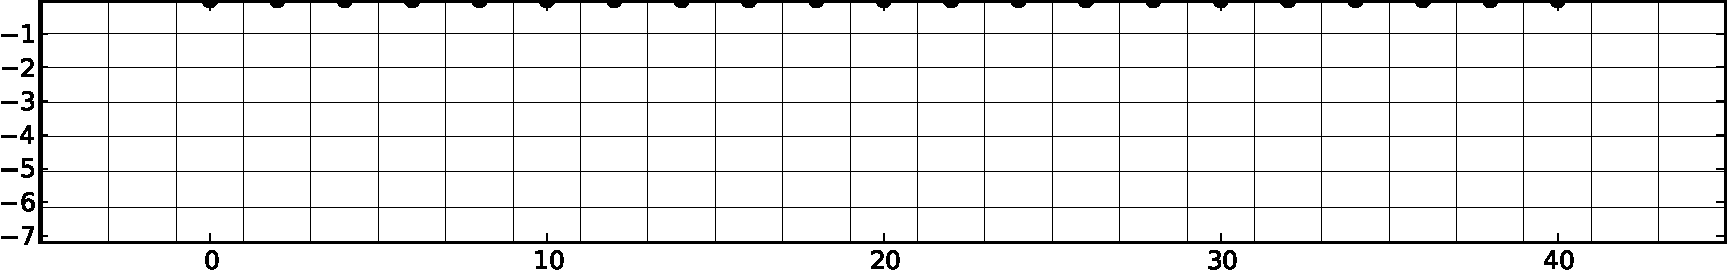
\includegraphics[width=0.45\textwidth]{structured2DMesh.pdf}\\
\centering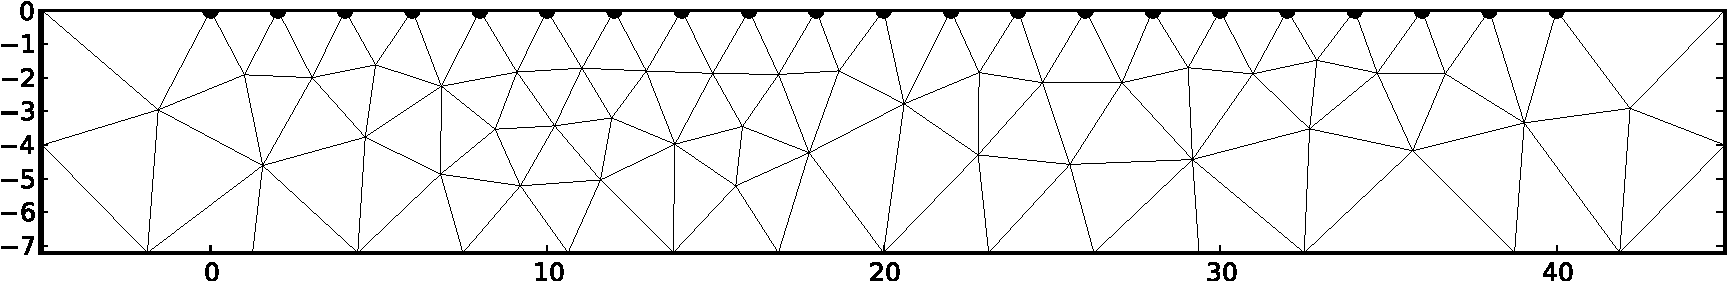
\includegraphics[width=0.45\textwidth]{unstructured2DMesh.pdf}\\
\centering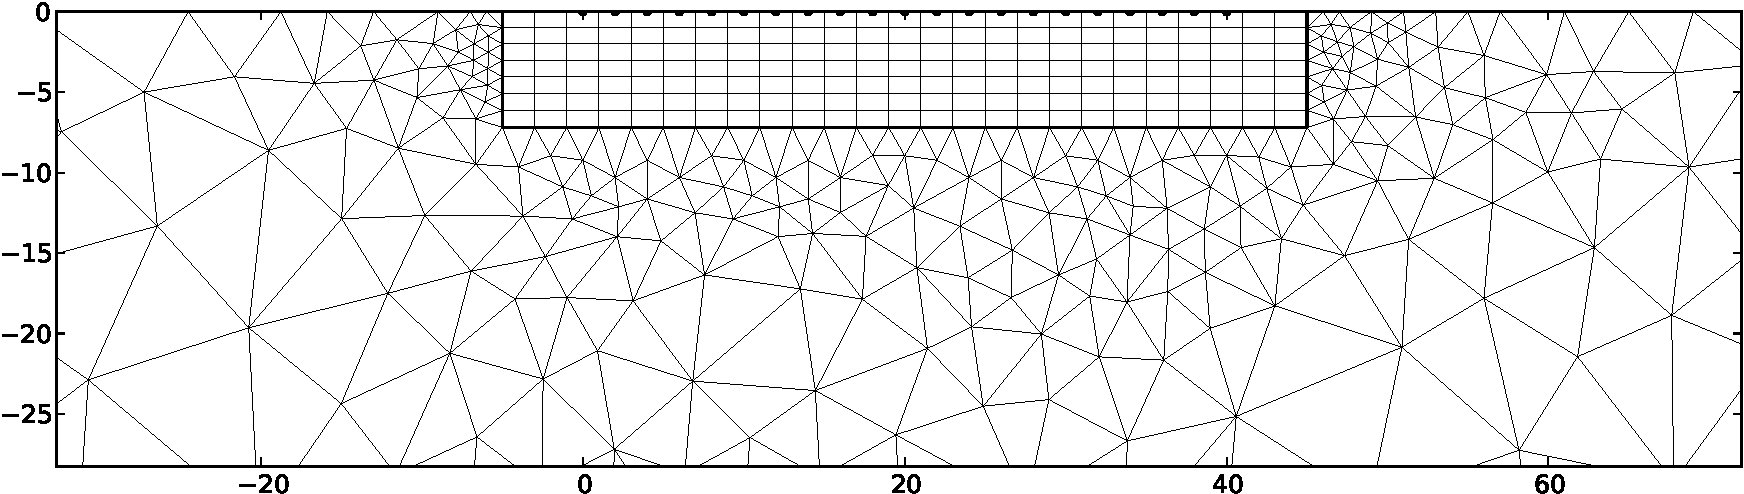
\includegraphics[width=0.45\textwidth]{mixed2DMesh.pdf}
\caption{Different parameterisations: 0d (independent parameters), 1d mesh, 2d structured mesh (grid), 2d unstructured mesh, 2d mixed mesh, 3d mesh}\label{fig:para}
\end{figure}

A combination of different data is easily achieved by the described error weighting and combining two vectors, e.g. amplitude and phase data in MT, in one vector.
Different parameters, can similarly be treated by different parts of the model vector, so-called regions.
Regions can be, as the name states, parts of one mesh representing different geological units.
Regions can also be different parameters on the same mesh (e.g. porosity and saturation) or on different parametrisations, e.g. a 2d/3d resistivity distribution and (0d) values for static shift in MT inversion.

In inversion the regions are by default independent from each other, but can as well be constrained to another.
For each region the starting model value, but also constraint type, model and constraint control and the used transformation function can be freely defined.
Special regions are a background region (not part of inversion) and a single-parameter region (all cells a compounded to one parameter). See appendix \ref{app:regions} for how to control the behaviour of regions.

%%%%%%%%%%%%%%%%%%%%%%%%%%%%%%%%%%%%%%%%%%%%%%%%%%%%%%%%%%%%%%%%%%%%%%%%%%%
\subsection{Obtaining and building GIMLi}
Since summer 2011, GIMLi is hosted on SourceForge under the project name libgimli\footnote{Note that since this change the BERT components were excluded from the project to a dedicated repository.}.
See \url{http://sourceforge.net/projects/libgimli/} for additional information such as binary downloads, documentation, bug tracker and feature request.
The code itself can be retrieved using subversion (SVN) using the address \url{https://libgimli.svn.sourceforge.net/svnroot/libgimli}.
As usual the code contains a current development (trunk), experimental changes or side-projects (branches) and stable versions (tags).

The main code is located under \file{src} and applications in different sub-folders under \file{apps}.
Under \file{doc} you will find Doxygen documentation and this tutorial including its code examples.
To build the binaries, the GNU build system (Autotools) is used: first, the script \cw{autogen.sh} runs the GNU autotools including \cw{configure} and \cw{make} runs the compilation.
The configuration tries to detect the necessary libraries, i.e. 
\begin{itemize}
	\item LAPACK (Linear algebra package) and BLAS (basic linear algebra subprograms), see \url{www.netlib.org}
	\item Boost C++ libraries (\url{boost.org}), we use multithreading and python bindings 
	\item SuiteSparse for solving sparse matrix systems (\url{http://www.cise.ufl.edu/research/sparse/SuiteSparse/}), we use Cholmod for symmetric matrices
\end{itemize}
Whereas LAPACK/BLAS and Boost can be made system-wide available on Linux systems using a package manager, SuiteSparse must be downloaded and built by hand. 
In the folder \file{external} there is a Makefile that tries to download and build LAPACK, BLAS and SuiteSparse.
All libraries should be located in \file{external/lib}, 
On Windows systems, you can use ready-compiled dll files.

For reasons of platform-compatibility, our codes are adapted to the GNU compilers but should be working with any compiler suite.
Whereas the GNU compiler collection is installed on any Linux or Mac system, on Windows MinGW (Minimalistic GNU for Windows, \url{www.mingw.org}) should be installed first.
For Windows we also recommend to use CodeBlocks as compiler IDE for which we prepared project files (\file{**.cbp}) in the folder \file{mingw}.

\subsubsection*{PyGIMLi}
Python (\url{www.python.org}) is a very powerful and easy-to-use programming language that combines the performance of numerical computation with high-end graphical output and user-interfaces.
We recommend PythonXY (\url{www.pythonxy.com}), a distribution coming along with a lot of modules for scientific computing and development environments such as Spyder.
The Python bindings for GIMLi, PyGIMLi, are located in the subfolder \file{python} make it very comfortable to write GIMLi applications.
In the folder \file{python} you find a build script \cw{build.sh} to build the binaries\footnote{The packages gccxml, pygccxml and pyplusplus are needen, but can also be retrieved using \cw{buildToolChain.sh} in the folder \file{buildScripts.sh}} as well as numerous other functions that can be used from python.

\subsubsection*{Installation}
Independent whether you use pre-compiled or self-build binaries the path to the executables, libraries and python modules must be known using the variables PATH, LD\_LIBRARY\_PATH\footnote{Under windows there is no differentiation and PATH is for both.} and PYTHONPATH.

%%%%%%%%%%%%%%%%%%%%%%%%%%%%%%%%%%%%%%%%%%%%%%%%%%%%%%%%%%%%%%%%%%%%%%%%%%%
\subsection{Outline of the document}\label{sec:overview}
In the following chapters we like to document how to work with the library using different examples.
A very simple example will illustrate how to setup a forward class and make the first inversion - polynomial curve fitting.
Then, some basic geophysical examples explain how parameterisations are used and options are set.
Three different joint inversion techniques are explained in the section \ref{sec:joint}.
The last section deals with the subject time-lapse inversion.
In the directory code there are the code examples used in the following.
